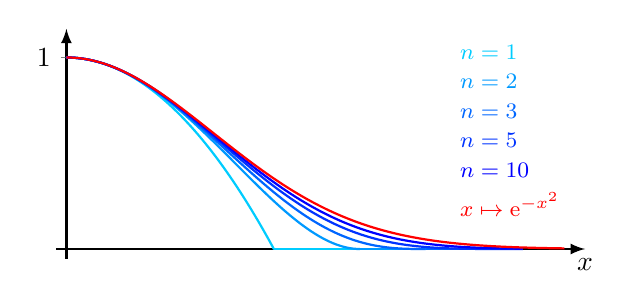
\begin{tikzpicture}
    \begin{axis}[
        width=8.3cm,
        height=4.5cm,        
        xmin=-0.05, xmax=2.5,
        ymin=-0.05, ymax=1.15,
        axis lines=middle,
        axis line style=thick,
        axis line style={-latex},
        legend cell align={left}, 
        legend style={
            draw=none,
            fill=none,
            font=\footnotesize,
            legend image code/.code={\node[anchor=west] {#1};}
        },
        xtick=\empty,
        ytick={0, 1},
        yticklabels={$0$, $1$},
        xlabel=$x$,
        every axis x label/.style={at={(current axis.right of origin)},anchor=north},
    ];

    % Plot for n=1
    \addplot[domain=0:sqrt(1), samples=200, color=blue!20!cyan, smooth, thick, line join=round,line cap=round] {(1 - (x^2)/1)^1};
    \addplot[domain=sqrt(1):2.2, samples=200, color=blue!20!cyan, smooth, thick] {0};
    \addlegendentry{\textcolor{blue!20!cyan}{$n = 1$}}

    % Plot for n=2
    \addplot[domain=0:sqrt(2), samples=200, color=blue!40!cyan, smooth, thick] {(1 - (x^2)/2)^2};
    \addplot[domain=sqrt(2):2.2, samples=200, color=blue!40!cyan, smooth, thick] {0};
    \addlegendentry{\textcolor{blue!40!cyan}{$n = 2$}}

    % Plot for n=3
    \addplot[domain=0:sqrt(3), samples=200, color=blue!60!cyan, smooth, thick] {(1 - (x^2)/3)^3};
    \addplot[domain=sqrt(3):2.2, samples=200, color=blue!60!cyan, smooth, thick] {0};
    \addlegendentry{\textcolor{blue!60!cyan}{$n = 3$}}

    % Plot for n=5
    \addplot[domain=0:2.2, samples=200, color=blue!80!cyan, smooth, thick] {(1 - (x^2)/5)^5};
    \addlegendentry{\textcolor{blue!80!cyan}{$n = 5$}}

    % Plot for n=10
    \addplot[domain=0:2.2, samples=200, color=blue!100!cyan, smooth, thick] {(1 - (x^2)/10)^10};
    \addlegendentry{\textcolor{blue!100!cyan}{$n = 10$}}

    % Plot for exponential function
    \addplot[domain=0:2.4, red, samples=200, smooth, thick] {exp(-x^2)};
    \addlegendentry{\textcolor{red}{$x \mapsto \mathrm{e}^{-x^2}$}}
    \end{axis}
\end{tikzpicture}
